\documentclass[answers]{exam}

%% Language and font encodings
\usepackage[spanish]{babel}
\usepackage[utf8x]{inputenc}
\usepackage[T1]{fontenc}

%% Sets page size and margins
\usepackage[a4paper,margin=2cm]{geometry}

%% Paquetes para listar código
\usepackage{xcolor}
\usepackage{listings}
\lstset{basicstyle=\ttfamily,
  showstringspaces=false,
  commentstyle=\color{red},
  keywordstyle=\color{blue}
}

%% Useful packages
\usepackage{amsmath}
\usepackage{graphicx}
\usepackage{paralist}
\usepackage{multicol} % Para las multicolumnas
\usepackage{hyperref} % Para links
\setlength\FrameSep{5pt}
\usepackage{amsmath}
\usepackage[ruled,vlined]{algorithm2e}
\DontPrintSemicolon
\newcommand{\To}{\mbox{\upshape\bfseries to}}
\pagestyle{empty} % Para quitar las páginas

\begin{document}
% --------------------------- Carátula --------------------------------
\begin{titlepage}
\begin{center}

{\huge \scshape Universidad Nacional Autónoma De México\\
Facultad de Ciencias\\\vspace{5mm} %5mm vertical space
Programación de Dispositivos Móviles, 2019-II}\\[1cm]

%----------------------------------------------------------------------------------------
%   TITLE SECTION
%----------------------------------------------------------------------------------------
\centering

\begin{center}
    
\includegraphics[width=17.5cm]{img/Android_Studio.jpg}\\[1cm]
\end{center}
\rule{0.8\textwidth}{.8pt}\\
{\huge \Huge \scshape Tarea 01: \\
\vspace{5mm}
\textit{Android Studio.}}\\
\rule{0.8\textwidth}{.8pt}

%----------------------------------------------------------------------------------------
%   AUTHOR SECTION
%----------------------------------------------------------------------------------------
\vspace{15mm} %5mm vertical space

{\huge \scshape Integrante:}\\
\vspace{5mm} %5mm vertical space
{\huge Sánchez Morales Rodrigo Alejandro.}\\ [1cm]

{\huge \scshape Profesora:}\\
\vspace{5mm} %5mm vertical space
{\huge Ana Libia Eslava Cervantes.}\\ [1cm]

{\huge \scshape Ayudante:}\\
\vspace{5mm} %5mm vertical space
{\huge Manuel Ignacio Castillo López.}\\ [1cm]

{\huge \scshape Fecha de entrega:}\\
\vspace{5mm} %5mm vertical space
{\huge 13 de Febrero del 2019.}\\[1cm]

\vfill % Fill the rest of the page with whitespace

\end{center}
\end{titlepage}

\begin{questions}

\question{\texttt{Android SDK.}}

\begin{framed}
    Deberá instalar o actualizar los siguientes paquetes:
    \begin{itemize}
        \item Android SDK Platform (al momento de redactar, la versión más reciente es Android 9.0 Pie, nivel de API 28, 6ta. revisión).
        \item Android SDK Build-Tools.
        \item Android Emulator.
        \item Android SDK Platform-Tools.
        \item Android SDK Tools.
        \item Google USB Driver (sólo Windows).
        \item Todos los paquetes del repositorio de soporte (Lista desplegable al final de la pestaña).
    \end{itemize}
    \textbf{Suba una captura de pantalla donde se muestre en el Android SDK Manager que estos paquetes están instalados.} \\ \\
    \begin{center}
        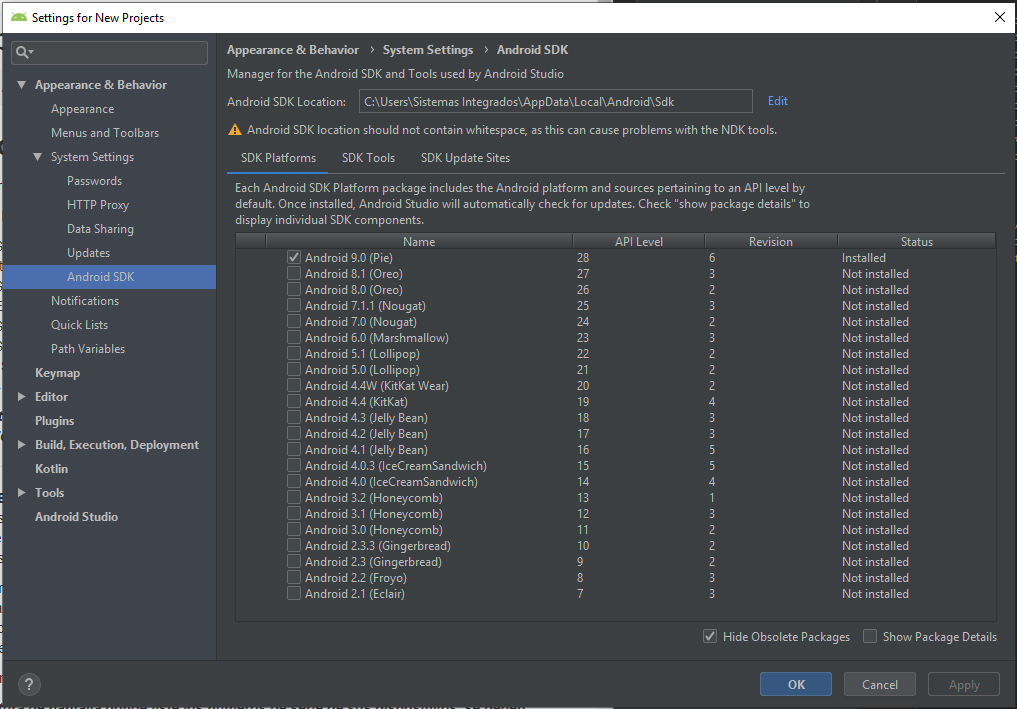
\includegraphics[width=15.5cm]{img/AndroidSDK_01.png}
    \end{center}
    \begin{center}
        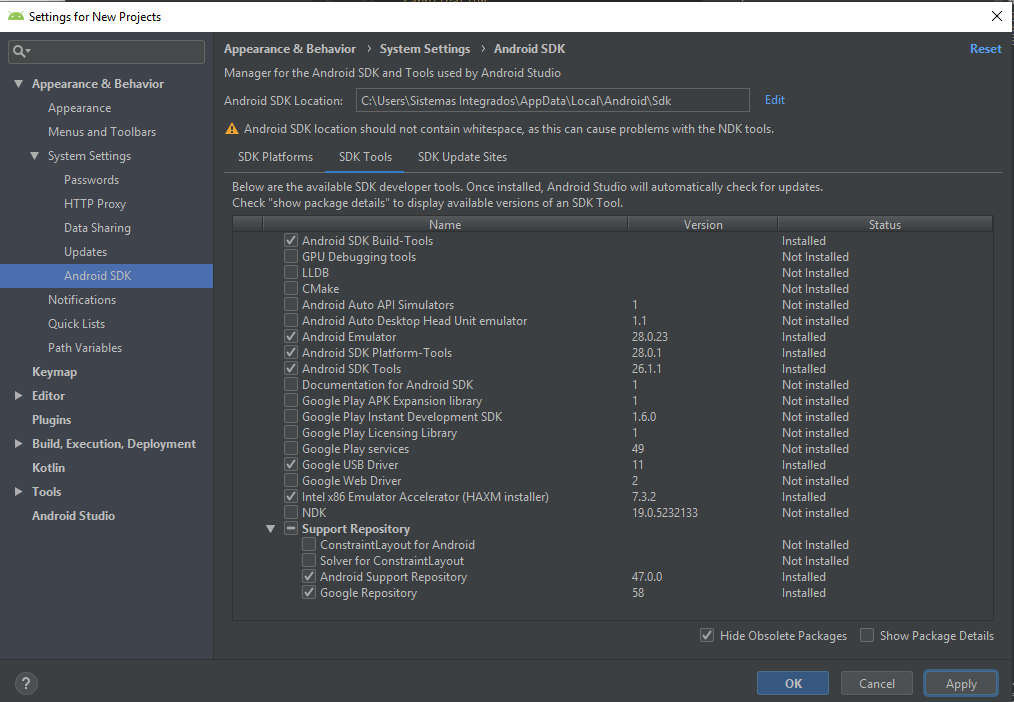
\includegraphics[width=15.5cm]{img/AndroidSDK_02.png}
    \end{center}
    \begin{center}
        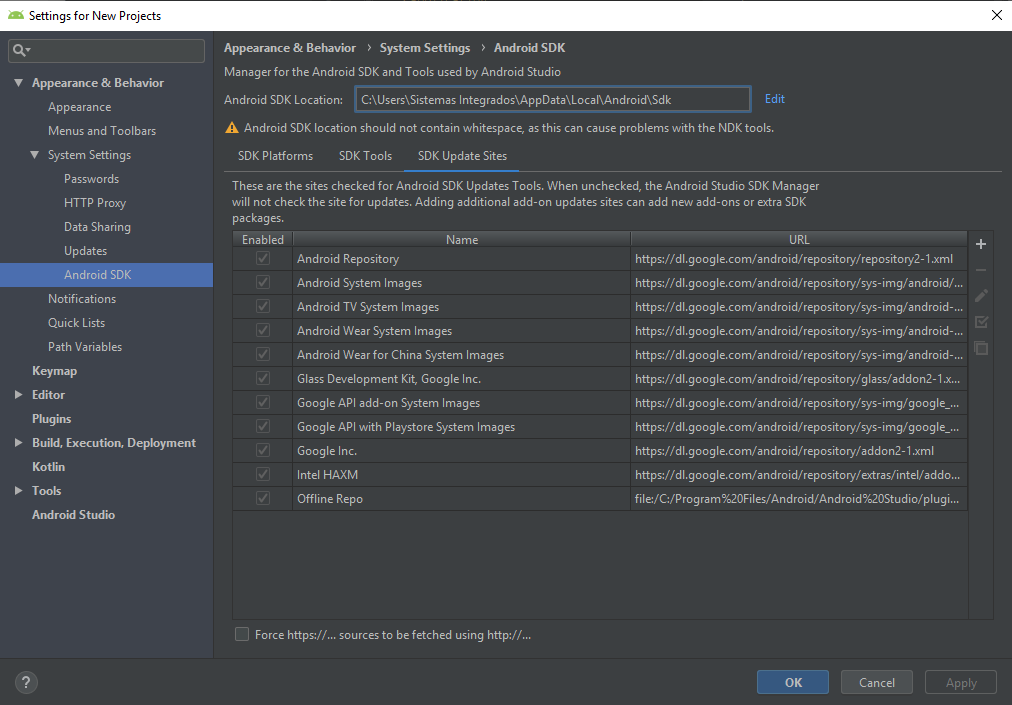
\includegraphics[width=15.5cm]{img/AndroidSDK_03.png}
    \end{center}
\end{framed}

\question{\texttt{Usando el ADB.}}

\begin{framed}
    En los dispositivos Android que vaya a usar para depurar sus aplicaciones, abra las configuraciones y vaya a Acerca del dispositivo y toque repetidas veces el campo Número de compilación hasta que se le indique que se ha activado el modo de desarrollador. Vuelva al menú principal de las configuraciones y ubique la opción desbloqueada Opciones de desarrollador y active la depuración USB.
    
    El equipo con \href{http://esie.icat.unam.mx/moodle/mod/folder/view.php?id=451}{Android Studio}. usando una consola inicie el ADB. Conecte uno o más dispositivos por USB al sistema; a los que previamente le ha activado la depuracion USB con el procedimiento anterior y liste los números de serie de los dispositivos. Cambie el estado de unauthorized a device, indicando que siempre va a permitir la depuración del equipo de desarrollo en el dispositivo de prueba.
    
    Finalmente, reinicie uno de los dispositivos usando el comando remoto reboot.
    
    \textbf{Suba una captura de pantalla donde liste los números de serie de sus dispositivos, se deben mostrar en estado device y no unauthorized.}
    
    \begin{center}
        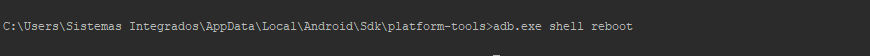
\includegraphics[width=15.5cm]{img/AndroidADB_01.png}
    \end{center}
    \begin{center}
        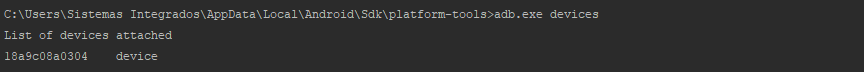
\includegraphics[width=15.5cm]{img/AndroidADB_02.png}
    \end{center}
\end{framed}

\question{\texttt{Android Virtual Device.}}

\begin{framed}
    Cree un dispositivo virtual de Android tipo teléfono y otro tipo tablet. El smartphone virtual debe contar con las siguientes características:
    
    \begin{itemize}
        \item Pantalla de 1080x1920 px
        \item Play Store.
        \item API nivel 28 (Android 9.0 Pie).
        \item Arquitectura x86
        \item 2 Gb de RAM
    \end{itemize}

    La tablet deberá contar con las siguientes características:
    
    \begin{itemize}
        \item Pantalla de densidad xhdpi.
        \item 2 Gb de RAM
        \item API nivel 19 (Android 4.4 Kitkat)
        \item Arquitectura x86
    \end{itemize}
    
    \textbf{Suba una captura de pantalla de ambos AVD en ejeución.}

    \begin{center}
        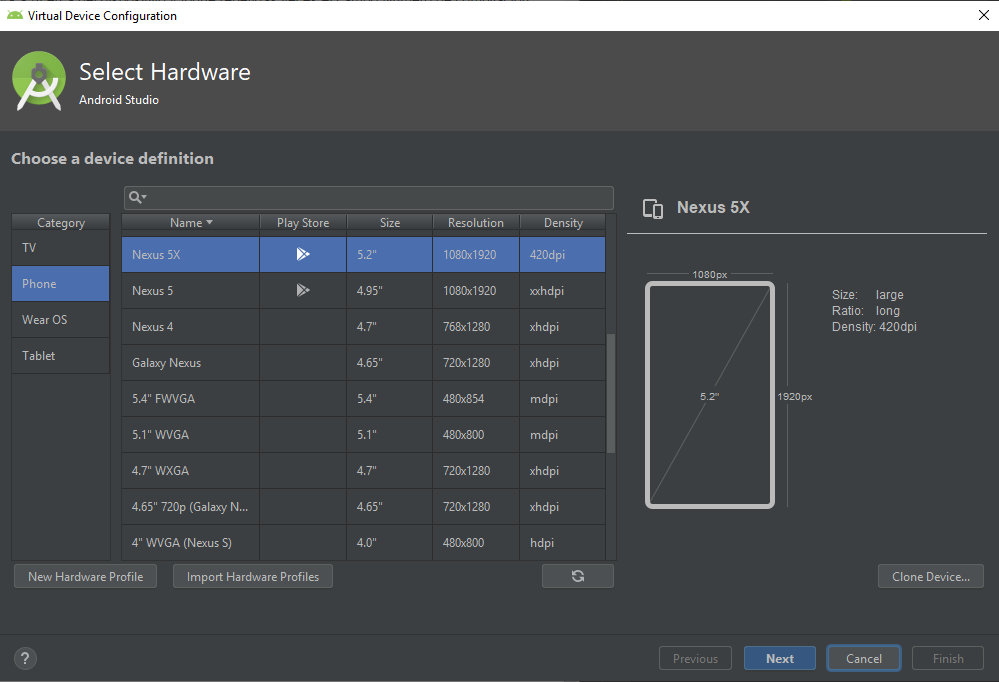
\includegraphics[width=15.5cm]{img/AndroidVirtualDevices_01.png}
    \end{center}
    \begin{center}
        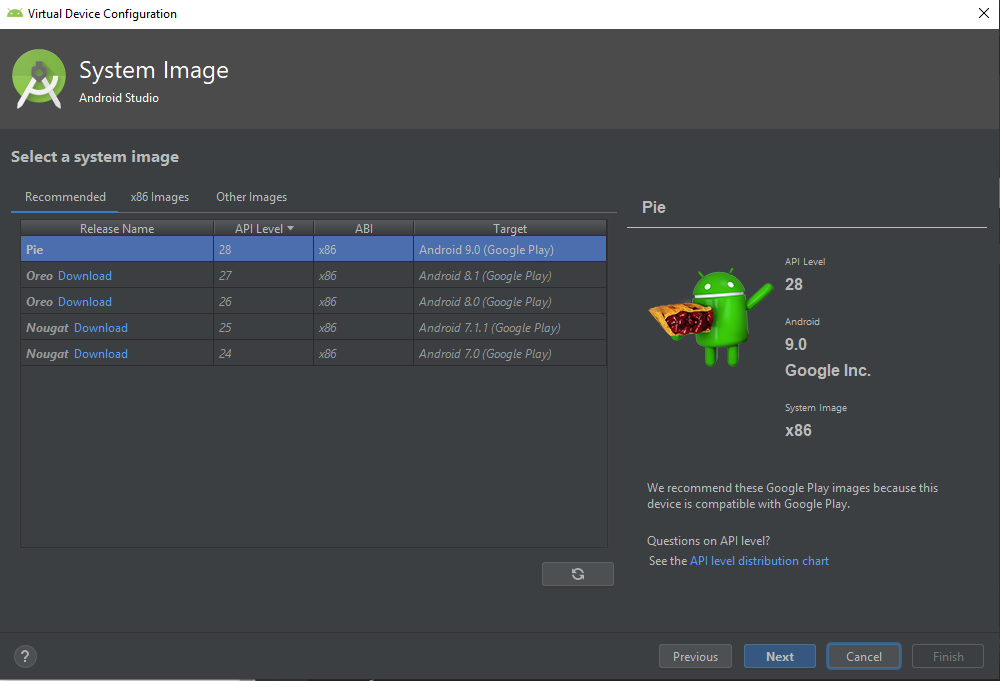
\includegraphics[width=15.5cm]{img/AndroidVirtualDevices_02.png}
    \end{center}
    \begin{center}
        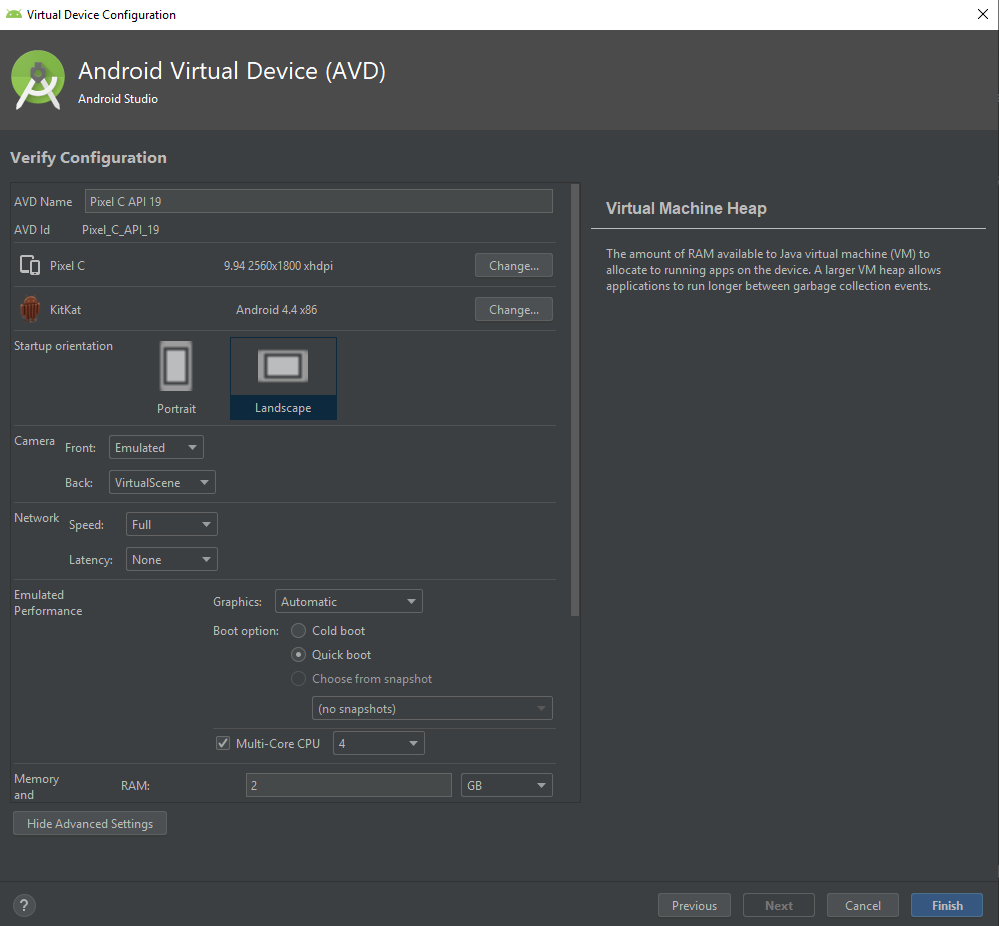
\includegraphics[width=15.5cm]{img/AndroidVirtualDevices_03.png}
    \end{center}
    \begin{center}
        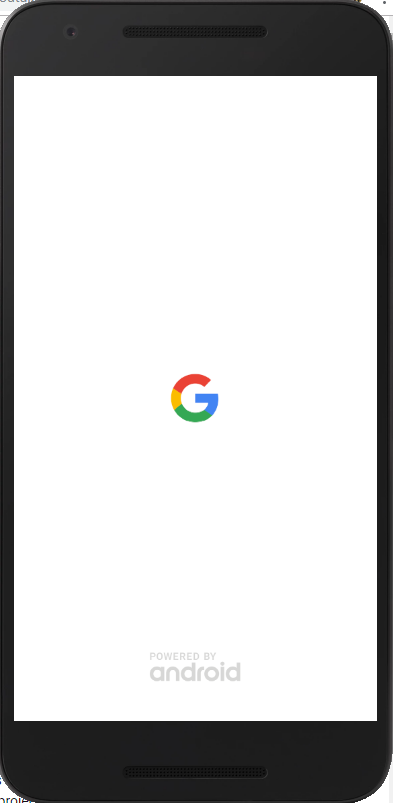
\includegraphics[height=10cm]{img/AndroidVirtualDevices_04.png}
        \hspace{1cm}
        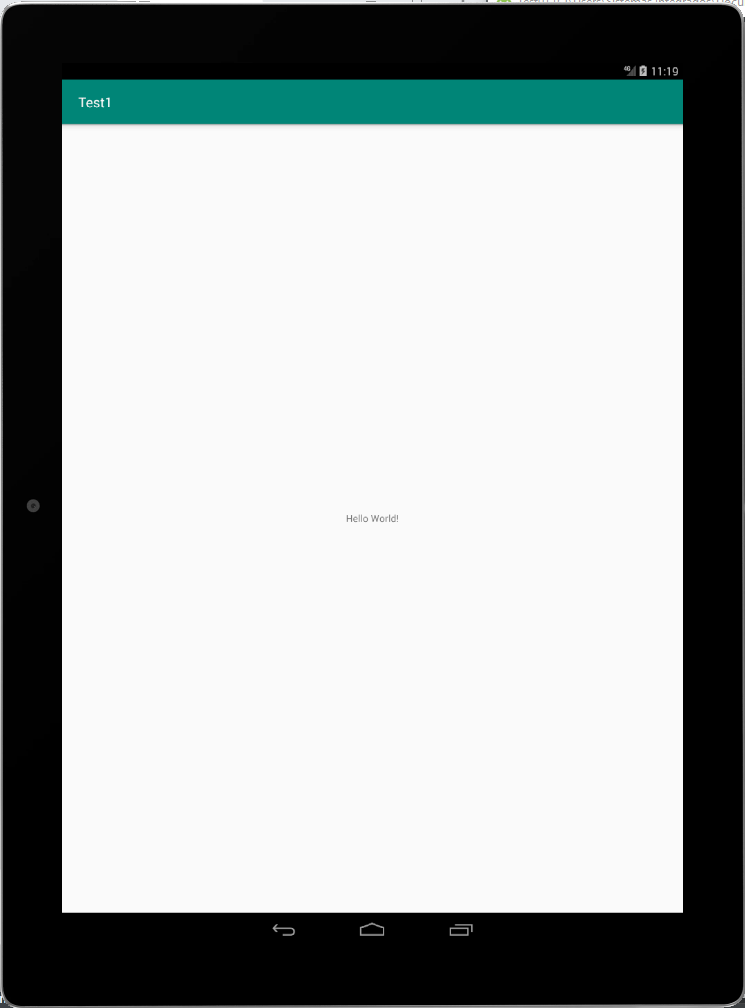
\includegraphics[height=10cm]{img/AndroidVirtualDevices_05.png}
    \end{center}
\end{framed}

\end{questions}
\end{document}